% $Id: VM_implnotes.tex,v 1.1 2004/05/17 17:39:51 theurich Exp $

%\subsection{Design and Implementation Notes}

The VM class provides an additional layer of abstraction on top of the POSIX machine model, making it suitable for HPC applications. There are four key aspects the VM class deals with.

\begin{enumerate}

\item Encapsulation of hardware and operating system details within the concept of Permanent Execution Threads (PETs).

\item Resource management in terms of PETs with a guard against oversubscription.

\item Topological description of the underlying configuration of the compute resources in terms of PETs.

\item Transparent communication API for point-to-point and collective PET-based primiteves, hiding the many different communication channels and offering best possible performance.

\end{enumerate}

%\begin{center}
%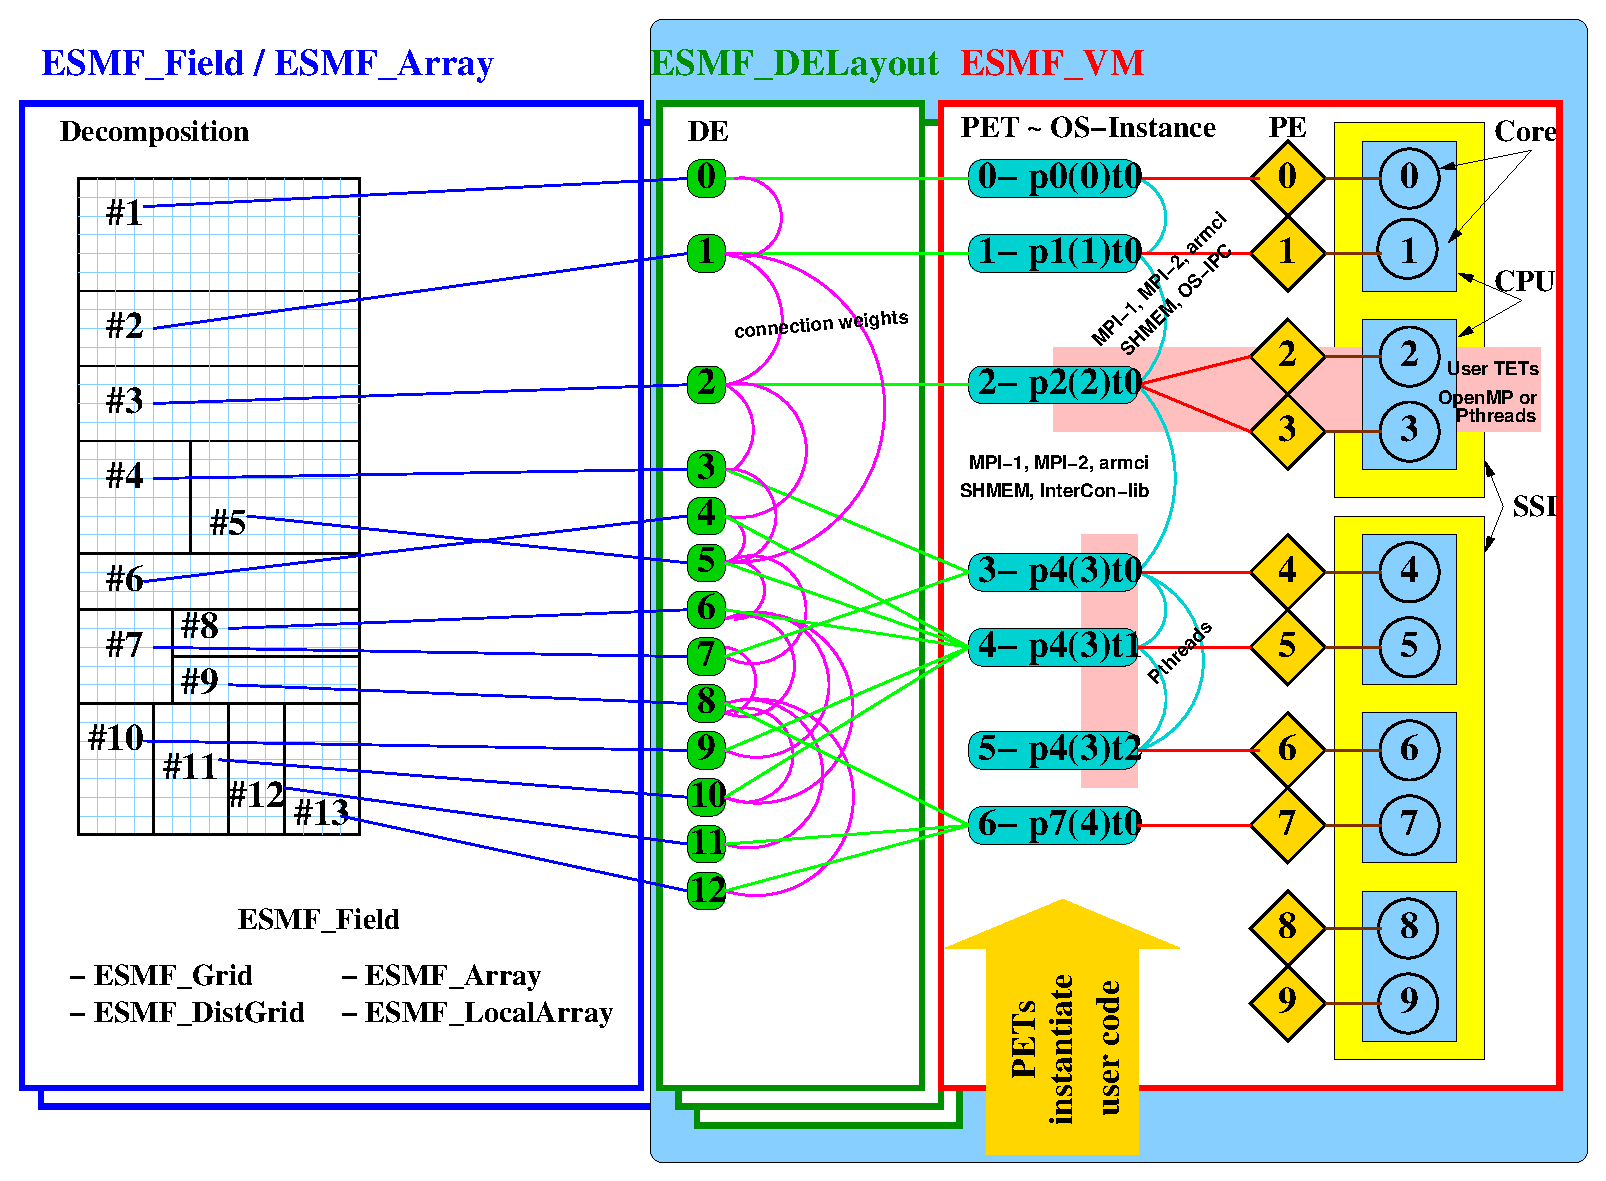
\includegraphics{VM_design.eps}
%\end{center}


{\bf Definition of terms used in the diagram}

\begin{itemize}

\item PE: A processing element (PE) is an alias for the smallest physical processing unit available on a particular hardware platform. In the language of today's microprocessor architecture technology a PE is identical to a core, however, if future microprocessor designs change the smallest physical processing unit the mapping of the PE to actual hardware will change accordingly. Thus the PE layer separates the hardware specific part of the VM from the hardware-independent part. Each PE is labeled with an id number which identifies it uniquely within all of the VM instances of an ESMF application.

\item Core: A Core is the smallest physical processing unit which typically comprises a register set, an integer arithmetic unit, a floating-point unit and various control units. Traditionally there was one core per CPU, however, today some dual-core CPUs are available and  multi-core CPU designs are on most manufacturers' road-maps. Each Core is labeled with an id number which identifies it uniquely within all of the VM instances of an ESMF application.

\item CPU: The central processing unit (CPU) houses single or multiple cores, providing them with the interface to system memory, interconnects and IO. Typically the CPU provides some level of caching for the instruction and data streams in and out of the Cores. Cores in a multi-core CPU typically share some caches. Each CPU is labeled with an id number which identifies it uniquely within all of the VM instances of an ESMF application.

\item SSI: A single system image (SSI) spans all the CPUs controlled by a single running instance of the operating system. SMP and NUMA are typical multi-CPU SSI architectures. Each SSI is labeled with an id number which identifies it uniquely within all of the VM instances of an ESMF application.

\item TOE: A thread of execution (TOE) executes an instruction sequence. TOE's come in two flavors: PET and TET.

\item PET: A permanent execution thread (PET) executes an instruction sequence on an associated set of data. The PET has a lifetime at least as long as the associated data set. In ESMF the PET is the central concept of abstraction provided by the VM class. The PETs of an VM object are labeled from 0 to N-1 where N is the total number of PETs in the VM object.

\item TET: A transient execution thread (TET) executes an instruction sequence on an associated set of data. A TET's lifetime might be shorter than that of the associated data set.

\item OS-Instance: The OS-Instance of a TOE describes how a particular TOE is instantiated on the OS level. Using POSIX terminology a TOE will run as a single thread within a single- or multi-threaded process.

\item Pthreads: Communication via the POSIX Thread interface.

\item MPI-1, MPI-2: Communication via MPI standards 1 and 2.

\item armci: Communication via the aggregate remote memory copy interface.

\item SHMEM: Communication via the SHMEM interface.

\item OS-IPC: Communication via the operating system's inter process communication interface. Either POSIX IPC or System V IPC.

\item InterCon-lib: Communication via the interconnect's library native interface. An example is the Elan library for Quadrics.

\end{itemize}

The POSIX machine abstraction, while a very powerful concept, needs augmentation when applied to HPC applications. Key elements of the POSIX abstraction are processes, which provide virtually unlimited resources (memory, I/O, sockets, ...) to possibly multiple threads of execution. Similarily POSIX threads create the illusion that there are virtually unlimited processing elements present and available to each POSIX process. While the POSIX abstraction is very suitable for many multi-user/multi-tasking applications that need to share limited physical resources, it does not directly fit the HPC workload where oversubscription of resources is one of the most expensive modes of operation.

The VM holds information on the available physical processing units in terms of Cores, CPUs and SSIs, which make up the physical machine layout, and provides a flat view of the physical machine by intoducing the PE (processing element) concept. A PE is the smallest physical processing unit available on a particular machine.

The key abstraction provided by the VM is the PET. All user code is executed by PETs while the OS details are hidden. The VM class contains a number of methods which allow the user to prescribe how the PETs of a desired virtual machine should be instantiated on the OS level and how they should map onto the hardware. This prescription is kept in a private virtual machine plan object which is being created at the same time the associated component is being created. Each time any component code is entered through the component's registered top--level methods (Initialize/Run/Finalize), the virtual machine plan along with a pointer to the respective user function is used to instantiate the user code on the PETs of the assiciated VM in form of single- or multi-threaded processes. 

The process of starting, entering, exiting and shutting down a VM is very transparent, all spawning and joining of threads is handled by VM methods "behind the scenes". Furthermore, fundamental synchronization and communication primitives are provided on the PET level through a uniform API, hiding details related to the actual PET OS-instantiation.

There is only one unique physical machine layout for each application, and all instances of the VM have access to this information. The PE is the smallest processing unit, which in today's microporcessor technology, corresponds to a single Core. Cores are arranged in CPUs and SSIs. The setup of the physical machine layout is part of the initialization of the default virtual machine which subscribs one PET, instantiated as single-threaded process, to each core. Using the physical machine layout it is possible to provide very generic virtual machine plan methods as well as guard against oversubscription.

Within one VM object each PE of the physical machine layout maps to 0 or 1 PETs. Allowing unassigned PEs provides a means to prevent oversubscription between multiple concurrently running virtual machines. Similarly a maximum of one PET per PE prevents oversubscription within a single VM instance. However, oversubscription is possible by subscribing PETs from different virtual machines to the same PE. This type of oversubscription can be desirable for PETs associated with IO work loads expected to be used infrequently and to block often on IO requests.

Each PET of a VM object maps to at least 1 PE of the physical machine layout, thus ensuring its execution. Mapping a single PET to multiple PEs provides resources for user-level multi-threading. The user code executing on the PET inquires how many PEs are associated with its PET and if there are multiple PEs available the user code can spawn an equal number of threads (e.g. OpenMP) without risking oversubscription. Typically these user spawned threads are short-lived and used for fine-grained parallelization in form of TETs. All PEs mapped against a single PET must be part of a unique SSI!

ESMF initialization sets up the default virtual machine with as many PETs, instantiated as single-threaded MPI processes, as there are PEs and uses a 1:1 mapping of PETs to PEs.

The user code executing during the registration call of a component may use an VMDef call to define its virtual machine. Internally this will create an VMPlan associated with this component. The default VMPlan defines an MPI-only VM.

Each time any component code is entered via Initialize, Run or Finalize ESMF will enter a virtual machine according to the assiociated plan and exit on return. Thus all component user code will be executed by the PETs of the prescribed virtual machine. The user code will be provided with a handle to the VM object. 

On the OS level all PETs are instantiated as Pthreads, either belonging to a group of threads running withing a multi-threaded process or as a single thread within a single-threaded process.

The number of processes is static during the course of execution and determined at start-up. The VM convention requires that the user starts up the ESMF application with as many MPI processes as there are PEs in the available physical machine. This is to mean that in case the user requested 8 dual-core CPUs from the system (e.g. via some queuing system), then the user should launch the ESMF application with 8 x 2 = 16 MPI processes.

All MPI processes participating in the set of PETs of a virtual machine are grouped together by a MPI\_Group object and their context is accessible via a MPI\_Comm object (MPI intra-communicator).

The PET local process id within each virtual machine is equal to the MPI\_Comm\_rank in the local MPI\_Comm object and the PET process id within each virtual machine is equal to the MPI\_Comm\_rank in the MPI\_COMM\_WORLD.
Within a ESMF component the virtual machine is "static". However, 
sub-components can define their own virtual machines within the
resources of their parent's virtual machine.




